\documentclass[a4paper, 11pt]{article}

\usepackage{graphicx}
\usepackage[brazil]{babel}
\usepackage[utf8]{inputenc}
\usepackage{epsfig}
\usepackage{float}
\usepackage{graphics}
\usepackage{url}
\usepackage[tight,footnotesize]{subfigure}
\usepackage{stfloats}
\usepackage{enumerate}
\usepackage[left=3cm,top=3cm,right=3cm,bottom=3cm]{geometry}

% correct bad hyphenation here
\hyphenation{op-tical net-works semi-conduc-tor}


\begin{document}


{
\begin{center}
{\LARGE \textbf{Arquitetura para Mitiga\c{c}\~{a}o de Ataques DDoS}}
\vskip 0.5cm
{\Large Cinara Menegazzo, Fernando Cezar Bernardelli, Fernando Gielow, Nadine
Lipa Pari}
\end{center}
}

\section{Introdu\c{c}\~{a}o}

% introduzir ataques DDoS e a importância do problema
Um ataque DDoS (\emph{Distributed Denial-of-Service})
 consiste, genericamente, da tentativa de tornar indisponíveis
os recursos oferecidos por alguma entidade \cite{Zhang:11}. Na Internet, este
tipo de ataque tem se tornado cada vez mais comum, visando \emph{websites} de
grandes empresas. Recentemente, houveram ataques aos \emph{websites} da Amazon,
do Paypal e da bandeira de cartões de crédito Visa \cite{Zuckerman:10,ddosatks},
que
acarretaram em grandes prejuízos à estas empresas.

Diversas dificuldades são encontradas ao se tentar mitigar os efeitos destes
ataques. Em servidores de hospedagem tradicionais, os recursos são limitados e,
assim, quando o número de requisições ultrapassa um patamar máximo, não há como
continuar respondendo efetivamente às requisições. Em abordagens mais avançadas,
como é o caso de hospedagem em \emph{clouds} \cite{Zhang:10}, tais ataques
acarretam na alocação de uma quantidade imensa de recursos, as vezes até mesmo
capazes de
suprir todas as requisições que chegam ao servidor, independente de serem
clientes legítimos ou atacantes. Embora esta abordagem consiga tratar ataques
DDoS para determinados limites, é uma abordagem custosa, pois todos os recursos
utilizados nesta tentativa de mitigação acarretar\~ao em custos
\cite{Soon:10}.

O trabalho \cite{Bakshi:10} prop\~oe tratar este cen\'ario de ataques através da
criação de uma nova instância da aplicação. Uma vez que um ataque DDoS é
detectado, a proposta busca detectar os atacantes através de PINGs -
caso um cliente suspeito de ser atacante não responder ao PING, ele é
considerado como um
atacante, de fato. Desta maneira, apenas os clientes que responderem ao PING
serão
redirecionados para a nova instância da aplicação. Entretanto, tal abordagem
depende da premissa que atacantes jamais responderão a PINGs e que clientes
genuínos sempre responderão, o que nem sempre condiz com a realidade.

%\section{Por que DDoS?}
%Dos artigos pesquisados com soluções sobre DDoS (\cite{Zhang:11, Zuckerman:10,
%Soon:10}), todos respondem um ataque dessa natureza com alocação de mais
%recursos. Esse ainda é um problema em aberto; como o DDoS é um ataque bruto,
%responder com a alocação de mais recursos funciona até um certo limite de
%tamanho do ataque. Para contornar a solução, o atacante precisa apenas aumentar
%o tamanho da rede que ele controla, tarefa simples segundo dados recentes sobre
%o crescimento de redes zumbi \cite{Chao:09}.


%A escolha deste tema é justificada, inicialmente, pela importância de se tratar
%este tipo de ataque. É cada vez mais comum a retaliação de grandes empresas
%através de ataques DDoS, que são de grande simplicidade e
%eficácia~\cite{ddosatks}. 


Cada vez mais, percebe-se a demanda por solu\c{c}\~oes que atendam
aplica\c{c}\~oes da Internet do futuro com sistemas complexos e robustos como
\emph{clouds}. Assuntos como ataques de DDoS ainda carecem de boas
solu\c{c}\~oes para este cen\'ario, pois o poder de
alocar recursos para suportar um ataque deste tipo agora torna-se
poss\'ivel, por\'em cresce tamb\'em os custos do usu\'ario por eles, o que
carateriza-se como eDDoS (\emph{economic} DDoS)~\cite{Soon:10}.
  
Apesar de ataques de DDoS j\'a serem bastante pesquisados e algumas propostas
de mitiga\c{c}\~ao j\'a terem sido divulgadas, ao se trabalhar em cen\'arios de
\emph{clouds} os aspectos de mitiga\c{c}\~ao ainda est\~ao em aberto, pois
apenas estender os recursos torna-se um recurso custoso e a melhor
solu\c{c}\~ao ainda dever\'a ser encontrada . Portanto, a mitiga\c{c}\~ao de
DDoS em \emph{clouds} ainda demandam pesquisas.


%ainda seja vulnerável a tais ataques. Ainda assim, foi observado
% que as soluções atuais convergem na vasta maioria para o tratamento de ataques
% através da maior alocação de recursos, impactando economicamente as empresas
% atacadas e não garantindo a efetiva mitigação dos ataques. As poucas soluções
% que não se baseiam inteiramente na maior alocação de recursos,
% como~\cite{Soon:10}, se mostraram inadequadas por premissas que nem sempre são
% verdadeiras.

\section{Objetivo}
Baseando-se no cen\'ario de problemas levantado na introdu\c{c}\~{a}o, este
trabalho de pesquisa gerar\'a uma arquitetura para mitigação de ataques de
DDoS executados sobre uma aplicação hospedada em uma \emph{cloud}. Esta
arquitetura, dever\'a monitorar o tr\'afego da aplica\c{c}\~{a}o e quando
detectar
ocorrência de ataque de DDoS, ser\'a respons\'avel por instanciar uma nova
instância desta
aplica\c{c}\~{a}o, garantindo que nenhum tr\'afego malicioso a alcance.

Esta arquitetura será composta pelos módulos abaixo e é ilustrada na
Figura~\ref{fig:arq}, onde diferentes inst\^ancias de servidores na nuvem s\~ao
representadas pelas caixas cinzas.

\begin{enumerate}[i]
  \item analizador de tráfego;
  \item redirecionador de tráfego;
  \item gerenciador de \emph{blacklist};
  \item instanciador de nova aplica\c{c}\~{a}o.
\end{enumerate}

\begin{figure}[h!]
\centering
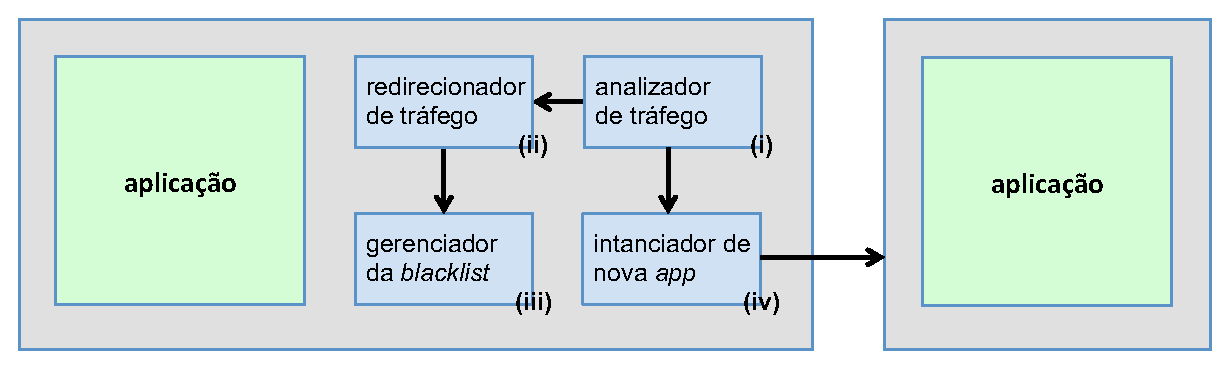
\includegraphics[width=0.85\textwidth]{arquitetura.eps}
\caption{Ilustração da proposta de arquitetura para mitigação de ataques DDoS}
\label{fig:arq}
\end{figure}

O módulo (i) observará proativamente o padrão de tráfego de entrada, visando
detectar um ataque DDoS. Caso um ataque seja detectado, o m\'odulo (iv) criará
uma nova
instância da aplicação em uma outra instância de servidor no \emph{cloud},
consequentemente com um endereço IP diferente.
Com isso, o módulo (ii) será responsável por tratar todo o tráfego de
entrada, informando o endereço do novo servidor, e inserindo o IP origem da
requisição à uma \emph{blacklist}, através do módulo (iii). Assim, o
atacante não afetará a nova instância da aplicação, pois ele não interpretará as
respostas que informam o IP da nova instância.


\section{Metodologia}
A pesquisa empregar\'a metodologia baseada em implementa\c{c}\~{a}o e medidas de
efici\^encia da solu\c{c}\~{a}o, que se propõem a mitigar o impacto causado pelo
tipo de ataque DDoS. Para que os objetivos sejam atingidos, a metodologia
dever\'a
compreender etapas como pesquisa bibliogr\'afica para levantamento de trabalhos
correlatos. Pela avalia\c{c}\~{a}o destes trabalhos ser\'a poss\'ivel
classificar as
solu\c{c}\~oes aplicadas tanto para detectar como para controlar ataques de
DDoS,
especificamente para ambientes de \emph{cloud}. Tendo como refer\^encia as
solu\c{c}\~oes aplicadas e os problemas ainda existentes, nosso trabalho
buscar\'a
alternativas capazes de efetivamente trazer melhorias ao problema levantado,
de acordo com a especificação da seção anterior.
Estas melhorias ser\~ao aplicadas em um ambiente real de \emph{cloud} como
Heroku~\cite{heroku}, Amazon~\cite{amazon}
ou Linode~\cite{linode} e monitoradas quanto a sua efici\^encia, considerando a
execu\c{c}a\~o correta da aplica\c{c}\~{a}o e o redirecionamento de apenas
requisições
confi\'aveis.


%\section{Proposta de Solu\c{c}\~{a}o}
%Inicialmente, nossa proposta compreender\'a o uso de tratamento de tr\'afego
%para identifica\c{c}\~{a}o de

%{\Large \textbf{Changeme!} }\emph{Será que não é melhor cortar essa seção?
%Seria muito redundante com a seção Objetivo..}

\section{Avalia\c{c}\~{a}o}
A etapa de avalia\c{c}\~{a}o da proposta consistirá principalmente na análise
da capacidade do servidor de atender novas requisições. Se o ataque de DDoS for devidamente
mitigado, as requisições de atacantes serão ignoradas, após eles serem introduzidos na \emph{blacklist}
e, assim, o servidor na \emph{cloud} deverá ser capaz de redirecionar apenas clientes legítimos 
para o novo servidor.

Com isso, para a análise, serão utilizadas ferramentas que geram requisições ao servidor. Como exemplos, o comando 
\emph{curl} pode ser utilizado em linha de comando para gerar uma requisição HTTP, sendo necessária a criação de \emph{scripts} mais robustos para incorporar diversas requisições. Outra alternativa é o uso do comando \emph{ab}, que permite a especificação do número de requisições que devem ser realizadas, a concorrência destas requisições, o tempo máximo que se deve esperar por respostas, e diversos outros parâmetros.

Como métricas, podemos utilizar o \textbf{tempo de resposta do servidor para requisições atendidas}, \textbf{taxa de requisições atendidas com relação ao número de clientes}, \textbf{carga gerada pelos módulos da arquitetura de acordo com o número de clientes}\footnote{note que o termo ``clientes'', aqui, engloba tanto clientes legítimos quanto atacantes.}. Novas métricas podem vir a serem consideradas, de acordo com a pesquisa que se sucederá.

\section{Etapas da Proposta}
\begin{itemize}
 \item Pesquisa
  \begin{itemize}
    % \item Levantamento de trabalhos relacionados
    \item Estudo de mecanismos para mitiga\c{c}\~{a}o de ataques DDoS
	\item Levantamento de métricas para análise de desempenho
	\item Pesquisa sobre algoritmos para detectar possíveis ataques DDoS
	\item Pesquisa sobre ferramentas para geração de requisições
  \end{itemize}

 \item Implementa\c{c}\~{a}o
  \begin{itemize}
      \item Módulo (i): analizador de tráfego;
	  \item Módulo (ii): redirecionador de tráfego;
	  \item Módulo (iii): gerenciador de \emph{blacklist};
	  \item Módulo (iv): instanciador de nova aplica\c{c}\~{a}o.
	  \item \emph{Dummy-application}
  \end{itemize}

 \item Teste de Desempenho 
  \begin{itemize}
    \item Definição de cenários
	\item Domínio das ferramentas para geração de requisições
	\item Realização da experimentação
	\item Análise dos resultados e elaboração de gráficos
  \end{itemize}
\end{itemize}


% \newpage
\bibliographystyle{unsrt}
\bibliography{proposta}
\end{document}
